\documentclass[11pt,a4paper]{article}
\usepackage[T1]{fontenc}
\usepackage[utf8]{inputenc}
\usepackage{lmodern}
\usepackage{amsmath,amssymb,amsthm,mathtools,mathrsfs}
\usepackage{graphicx,float,xcolor,multicol}
\usepackage[shortlabels]{enumitem}
\usepackage[margin=27mm]{geometry}
\usepackage{microtype,needspace,placeins}
\usepackage{tikz,tikz-cd}
\usetikzlibrary{arrows.meta,calc,positioning,patterns,decorations.pathreplacing}
\usepackage[colorlinks=true,linkcolor=teal,urlcolor=teal,citecolor=teal]{hyperref}
\setlength{\parindent}{0pt}
\setlength{\parskip}{.6em}
\setcounter{secnumdepth}{0}
\allowdisplaybreaks
\raggedbottom
\providecommand{\cross}{\times}
\DeclareUnicodeCharacter{2020}{\ensuremath{\dagger}}
\DeclareMathOperator{\supp}{supp}
\DeclareMathOperator*{\esssup}{ess\,sup}
\providecommand{\chapter}{\section}
\newenvironment{tool}[2]{\subsection*{Tool #1 --- #2}}{}
\newcommand{\ToolRef}[1]{Tool #1}
\newcommand{\FigureTag}[2]{\textit{Figure #1}}
\newcommand{\Result}[1]{\subsection*{#1}}
\newcommand{\Application}[1]{\subsubsection*{Application\if\relax\detokenize{#1}\relax\else\space--- #1\fi}}
\newcommand{\ProofHeading}{\par\textit{Proof.}\space}
\newcommand{\ProofOf}[1]{\par\textit{Proof of #1.}\space}
\newcommand{\RemarkHeading}{\par\textbf{Remark.}\space}
\newcommand{\NoteHeading}{\par\textbf{Note.}\space}
\newcommand{\ExerciseHeading}{\par\textbf{Exercise.}\space}

% Rendering support only; mathematical text is in each independent post.
\usepackage{booktabs,array,longtable}
\definecolor{HandoutBlue}{HTML}{2F6690}
\definecolor{HandoutNavy}{HTML}{17365D}
\newtheorem{theorem}{Theorem}
\newtheorem{lemma}[theorem]{Lemma}
\newtheorem{proposition}[theorem]{Proposition}
\newtheorem{corollary}[theorem]{Corollary}
\newtheorem{conjecture}[theorem]{Conjecture}
\newtheorem{definition}{Definition}
\newtheorem{example}{Example}
\newtheorem{namedtoolcounter}{Tool}
\newenvironment{namedtool}[1]{\begin{namedtoolcounter}[#1]}{\end{namedtoolcounter}}
\newtheorem*{claim}{Claim}
\newtheorem*{remark}{Remark}
\newtheorem*{exercise}{Exercise}
\newtheorem*{question}{Question}
\newtheorem*{observation}{Observation}
\newcommand{\SourceChapter}[2]{\section*{#2}}
\newcommand{\Lecture}[2]{\section*{Lecture #1: #2}}
\newcommand{\unclear}[1]{\textit{[unclear: #1]}}
\newcommand{\sourcegap}{\textit{[unfinished in the source]}}
\DeclareMathOperator{\dist}{dist}
\DeclareMathOperator{\id}{id}
\DeclareMathOperator{\Hol}{Hol}
\DeclareMathOperator{\Per}{Per}
\DeclareMathOperator{\Fix}{Fix}
\DeclareMathOperator{\diam}{diam}
\DeclareMathOperator{\Var}{Var}
\DeclareMathOperator{\Leb}{Leb}
\DeclareMathOperator{\Hom}{Hom}
\DeclareMathOperator{\End}{End}
\DeclareMathOperator{\Ann}{Ann}
\DeclareMathOperator{\Spec}{Spec}
\DeclareMathOperator{\Max}{Max}
\DeclareMathOperator{\Ob}{Ob}
\DeclareMathOperator{\Tor}{Tor}
\DeclareMathOperator{\Ass}{Ass}
\DeclareMathOperator{\Mor}{Mor}
\DeclareMathOperator{\Fun}{Fun}
\DeclareMathOperator{\Nat}{Nat}
\DeclareMathOperator{\Cone}{Cone}
\DeclareMathOperator{\MCG}{MCG}
\DeclareMathOperator{\Aut}{Aut}
\DeclareMathOperator{\Deck}{Deck}
\DeclareMathOperator{\SL}{SL}
\DeclareMathOperator{\PSL}{PSL}
\DeclareMathOperator{\Area}{Area}
\DeclareMathOperator{\im}{im}
\DeclareMathOperator{\PSh}{PSh}
\newcommand{\CRing}{\mathsf{CRings}}
\newcommand{\AMod}{A\text{-}\mathsf{Mod}}
\newcommand{\Ab}{\mathsf{Ab}}
\newcommand{\Z}{\mathbb Z}
\newcommand{\Q}{\mathbb Q}
\newcommand{\R}{\mathbb R}
\newcommand{\C}{\mathbb C}
\newcommand{\N}{\mathbb N}
\newcommand{\kk}{\mathbb k}
\renewcommand{\aa}{\mathfrak a}
\newcommand{\bb}{\mathfrak b}
\newcommand{\pp}{\mathfrak p}
\newcommand{\qq}{\mathfrak q}
\newcommand{\mm}{\mathfrak m}
\newcommand{\nn}{\mathfrak n}
\newcommand{\rad}{\mathrm r}
\newcommand{\cat}[1]{\mathsf{#1}}
\setcounter{secnumdepth}{0}
\allowdisplaybreaks

\graphicspath{{figures/commutative-algebra/}}
\begin{document}
\section*{Modules, Tensor Products, and the Determinant Trick}
% BLOG-CONTENT-BEGIN
\subsection{Modules}
\setcounter{example}{3}\begin{example}
\begin{enumerate}[label=(\roman*)]
\setcounter{enumi}{0}\item Ideals of $A$ are $A$-modules.
\setcounter{enumi}{1}\item $G\in\Ob(\mathsf{AbGps})$ is a $\Z$-module.
\setcounter{enumi}{2}\item A $\kk$-vector space is a $\kk$-module.
\setcounter{enumi}{3}\item If $M'\subseteq M$ are $A$-modules, then so is $M/M'$.
\setcounter{enumi}{4}\item If $\{M_i\}_{i\in I}$ are $A$-submodules of $M$, then so is $\sum_{i\in I}M_i$, defined analogously to the sum of ideals.
\setcounter{enumi}{5}\item Products and coproducts exist in the category of $A$-modules. Thus, if the $M_i$ are $A$-modules, so are $\bigoplus_{i\in I}M_i$ (direct sum) and $\prod_{i\in I}M_i$ (direct product).
\end{enumerate}
\end{example}
\setcounter{definition}{4}\begin{definition}
A map $f:M\to M'$ between $A$-modules is a \emph{module homomorphism} if
% Source page 12
$f\in\Hom_{\Ab}(M,M')$ and $f(ax)=af(x)$. Thus $f$ is equivariant with the ring action of $A$ on $M,M'$.
\end{definition}
% Source page 13
\subsection{Tensor products}
If $M,N$ are $A$-modules, there is a universal object among all $A$-bilinear maps from $M\times N$ to $P$, denoted $M\otimes N$. Thus $f:M\times N\to P$ factors through an $A$-linear map $\widetilde f$, as shown.
\begin{figure}[H]\centering
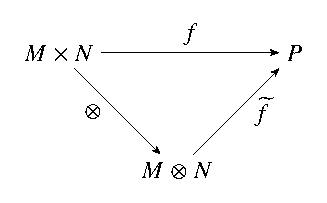
\includegraphics[width=.37\textwidth]{ca1-fig-06.pdf}
\FigureTag{CA1.6}{fig:ca-1-06}
\end{figure}
\paragraph{Construction.}
Consider the direct sum $\bigoplus_{i\in M\times N}A$. Let $C$ be the submodule generated by
\[
\begin{gathered}
(x+x',y)-(x,y)-(x',y),\qquad (x,y+y')-(x,y)-(x,y'),\\
(ax,y)-a(x,y),\qquad(x,ay)-a(x,y).
\end{gathered}
\]
Then $M\otimes N:=\bigl(\bigoplus_{i\in M\times N}A\bigr)/C$.
% The quotient is handwritten above the tensor-product paragraph; the later repeated definition is blank.
It is easy to check that $-\otimes N:\AMod\to\AMod$ and $N\otimes-:\AMod\to\AMod$ are functors. The source records the map $\Psi(f):(x,y)\mapsto f(x)(y)$.
\begin{claim}
\[\Hom(M\otimes N,P)\cong\Hom(M,\Hom(N,P)).\]
\end{claim}
\begin{claim}
The tensor-product functors above are right exact.
\end{claim}
\subsection{Finitely generated modules}
\setcounter{definition}{5}\begin{definition}
The module $M$ is \emph{free} if $M=\bigoplus_i A$.
\end{definition}
The source also records $A\otimes_A A\cong A$, $A/\aa\otimes_A A\cong A/\aa$.
\setcounter{definition}{6}\begin{definition}
$N$ is \emph{flat} if $-\otimes N$ is an exact functor.
\end{definition}
\setcounter{theorem}{3}\begin{theorem}[Cayley--Hamilton]
Let $M$ be a finitely generated $A$-module, $\varphi\in\End_{\AMod}(M)$, and $\varphi(M)\subseteq\aa M$, where $\aa$ is an ideal of $A$. Then
\[
\varphi^n+a_1\varphi^{n-1}+\cdots+a_n=0
\]
% Source page 15
for some $a_i\in\aa$, $n>0$.
\end{theorem}
\setcounter{theorem}{4}\begin{lemma}[Nakayama]
Let $M,\aa$ be as before. If $\aa\subseteq\bigcap_{\mm\text{ maximal}}\mm$ (the Jacobson radical) and $M=\aa M$, then $M=0$.
\end{lemma}
\begin{proof}
Cayley--Hamilton for $\varphi=\id$ yields, for $x=1+a_1+\cdots+a_n\equiv1\pmod\aa$, that $xM=0$. Since $x\equiv1\pmod\aa$,
\[
1-x\in\bigcap_{\mm\text{ maximal}}\mm
\ \Longrightarrow\ (1-x)\in\mm\ \text{for every maximal }\mm
\ \Longrightarrow\ x\in\mm^c\ \text{for every maximal }\mm.
\]
Hence $x$ is a unit. Therefore $M=x^{-1}(xM)=0$.
\end{proof}
% BLOG-CONTENT-END
\end{document}
